% Mirror: https://github.com/SIGma-UIUC/presentation-format
% --------------------------------------------------------------------
% This is a simple Beamer document that uses beamerthemesigma.sty
% Reading the comments should help you create a presentation even if
% you've never used Beamer before.
% --------------------------------------------------------------------

% Set our document class to Beamer
\documentclass[aspectratio=169]{beamer}
% \documentclass[aspectratio=169, handout]{beamer}
% Add handout option to ignore pauses

% From Jeff E
\usepackage{algo}
% Some more macros
\usepackage{sigmastyle}


% Set a title
\title{Complexity \& Fine-Grained Complexity}

% Set a subtitle if you desire
% \subtitle{[TAOCP 5 8.9.10.11]}

% Whoever worked on the presentation:
\author{Sam Ruggerio}

% Date looks ugly, so leave blank
\date{}

% An institute name, if you're so inclined
% \institute{University of Illinois Urbana-Champaign}

% Use the SIGma theme for this Beamer presentation
\usetheme{sigma}
% --------------------------------------------------------------------

% Begin document
\begin{document}

% Beamer calls each slide a "frame", defined within the environment:
% \begin{frame}
%   <frame content here>
% \end{frame}

% This frame is just the title.
\begin{frame}
\titlepage
\end{frame}

% A frame with the table of contents.
% This frame's title is "Outline".
% \begin{frame}{Outline}
%   \tableofcontents
% \end{frame}

\begin{frame}{Fine Grained Complexity}
    \begin{itemize}
        \item What is Computational Complexity?
        \item What are reductions?
        \item What is FGC?
        \item What do people research in FGC?
    \end{itemize}
\end{frame}

\begin{frame}{Complexity Primer}
    \begin{itemize}
        \item How do we determine the \textit{difficulty} of a problem? \pause
        \item There are many intuitive ways - but we're computer scientists! \pause
        \item Determine difficulty based on the runtime of an algorithm that solves the problem. \pause
        \item But what is our ground truth of computation? How do we know we have the best algorithm?
    \end{itemize}
\end{frame}

\begin{frame}{Complexity Primer}
    \begin{itemize}
        \item Sometimes we don't know the best algorithm! \pause
        \item We can still prove difficulty - just via other means. \pause
        \item However, we will sometimes need to choose a \textit{model of computation} as well.
    \end{itemize}
\end{frame}


\begin{frame}{Runtime Symbols}
    \begin{itemize}
        \item $O(f(n))$, some function $g(n) \in O(f(n))$ if $g(n)$ grows as much or no faster than $f(n)$ \pause
        \begin{itemize}
            \item $O(n)$ grows linearly w.r.t $n$. $O(n^2)$ grows quadratically. \pause
            \item $n \log (n) \in O(n^2)$ because it does not grow faster than $O(n^2)$. It is not in $O(n)$. \pause
        \end{itemize}
        \item $\Theta(f(n))$, ... "grows as-fast-as" ... ("Tight") \pause
        \item $\Omega(f(n))$, ... "grows at-least as fast as"  ("Lower Bound")
    \end{itemize}
\end{frame}

\begin{frame}{\small{Runtime Symbols}}
    \begin{itemize}
        \item $o(f(n))$, some function $g(n) \in o(f(n))$ if $g(n)$ grows strictly less than $f(n)$ \pause
        \begin{itemize}
            \item $n^2 \in O(n^2)$, but $n^2 \not \in o(n^2)$ \pause
            \item This is useful because we can say $n^{1.99999999} \in o(n^2)$ without needing specifics. \pause
        \end{itemize}
        \item $\omega(f(n))$, ... "grows strictly faster than" ...  ("Lower Bound")
    \end{itemize}
\end{frame}

\begin{frame}{Runtime Summary}
    \begin{itemize}
        \item You can view these Runtime Notations as (roughly) inequalities:
        \begin{itemize}
            \item $g(n) \in O( f(n) ) \iff g(n) \leq f(n)$
            \item $g(n) \in  o( f(n) ) \iff g(n) < f(n)$
            \item $g(n) \in  \Theta( f(n) ) \iff g(n) = f(n)$
            \item $g(n) \in  \omega( f(n)) \iff g(n) > f(n)$
            \item $g(n) \in \Omega(f(n)) \iff g(n) \geq f(n)$
        \end{itemize}
        \item But remember that these still abstract away constants and lower-order terms.
    \end{itemize}
\end{frame}

\begin{frame}{Lower Bound Example 1}
    \begin{itemize}
        \item How do we know that taking the min of $n$ elements needs to take at least $\Omega(n)$ time? \pause
        \item We proceed on contradiction:
        \begin{itemize}
            \item Assume we have an \textit{min}$()$ algorithm which runs in $o(n)$ \pause
            \item Then there must be some element we didn't observe... \pause 
            \item Thus, adversarialy that element can be the minimum, so no such algorithm exists! \pause
        \end{itemize}
        \item So $\textit{min}() \in \Omega(n)$
    \end{itemize}
\end{frame}

\begin{frame}{Lower Bound Example 2}
    \begin{itemize}
        \item How do we know that sorting is $\Omega(n \log n)$? \pause
        \item In this case, we change our model of computation to a model of \textit{decision trees} \pause
        \item The only operation we have available is to compare two elements and make new decisions. \pause
        \item This is very different from how we program, or even think about Turing machines.
    \end{itemize}
\end{frame}

\begin{frame}{Lower Bound Example 2}
  \begin{center}
    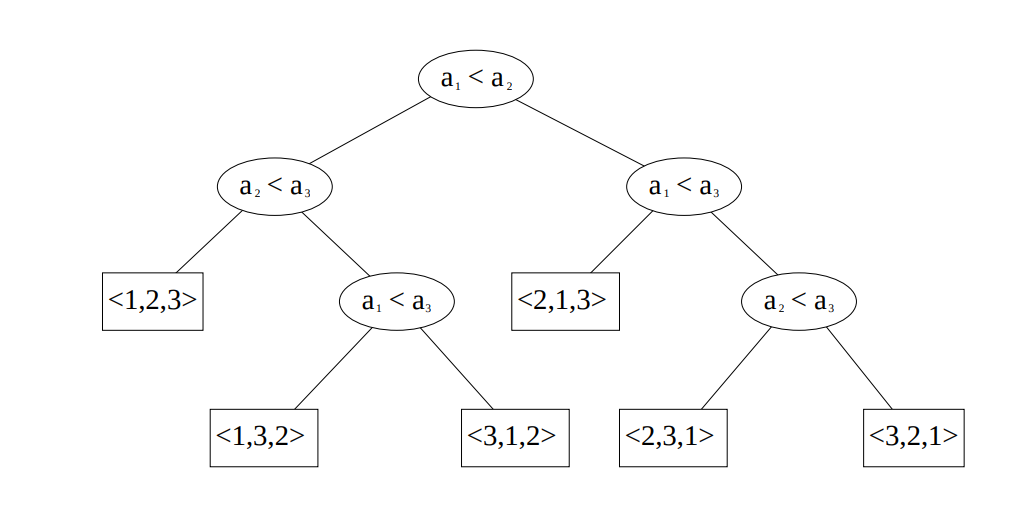
\includegraphics[width=\textwidth]{decision_tree.png}
  \end{center}
\end{frame}

\begin{frame}{Lower Bound Example 2}
    \begin{itemize}
        \item There are $n!$ possible permutations, thus $n!$ possible leaves \pause
        \item A tree of height $h$ has at most $2^h$ leaves \pause
        \item We find an $h$ such that $2^h \geq n!$ \pause
        \item $\log(2^h) \geq \log(n!) \implies h \geq n \log(n)$ \pause
        \item Thus sorting $n$ elements is $\Omega(n \log(n))$
    \end{itemize}
\end{frame}

\begin{frame}{P, NP, \& More}
    \begin{itemize}
        \item The first week we talked about P vs NP \pause
        \item P are problems \textit{decidable} in polynomial time \pause 
        \item NP are problems \textit{decidable} in non-deterministic, polynomial time \pause
        \begin{itemize}
            \item You can view non-determinism as always-perfect guessing or infinite multithreading \pause
            \item The equivalent definition is problems whose solutions can be checked in polynomial time
        \end{itemize}
    \end{itemize}
\end{frame}

\begin{frame}{P, NP, \& More}
    \begin{itemize}
        \item We know, via the Cook-Levin Theorem that Boolean Satisfiability is NP-Complete. \pause 
        \item This means it is representatively hard for all problems in NP \pause 
        \item These problems are also exponentially hard, i.e. runtimes on the order of $O(2^n)$. \pause
        \item This is not very useful to try and compute for any reasonable size
    \end{itemize}
\end{frame}

\begin{frame}{P, NP, \& More}
    \begin{itemize}
        \item We don't know if these problems have lower bounds that are not exponential (P vs NP) \pause
        \item If we have a hunch a problem is hard, how do we prove it? \pause
        \item Cook-Levin is a given, but its proof is tedious and complex to replicate for other problem types. \pause
        \item We can bypass this tediousness with reductions!
    \end{itemize}
\end{frame}


\begin{frame}{Reductions}
    \begin{itemize}
        \item We can show a problem is \textit{just as hard as} another problem by reducing a known hard problem to our target problem. \pause
        \item Let $A$ be our NP-Hard problem and $B$ be our target problem. \pause
        \item We're given an instance of $A$, e.g. if we had an algorithm for $A$, this would be the input. \pause
        \begin{itemize}
            \item Boolean Formula, Graph, etc.
        \end{itemize}
        \item We take that instance of $A$ and design an algorithm to convert it to an instance of $B$ \pause
        \item We this conversion to ensure that if we were to answer $A$ one way, we answer $B$ the same way. \pause
    \end{itemize}
\end{frame}

\begin{frame}{Reductions}
    \begin{itemize}
        \item Now given this conversion, we assume if we had a \textit{fast} algorithm for $B$, then this could imply a \textit{fast} algorithm for $A$ \pause
        \item As long as the runtime of our converter algorithm is polynomial (for NP-Hard reductions), this is a valid claim. \pause
        \item Since $A$ was NP-Hard, we now know that $B$ must be NP-Hard
    \end{itemize}
    \begin{center}
        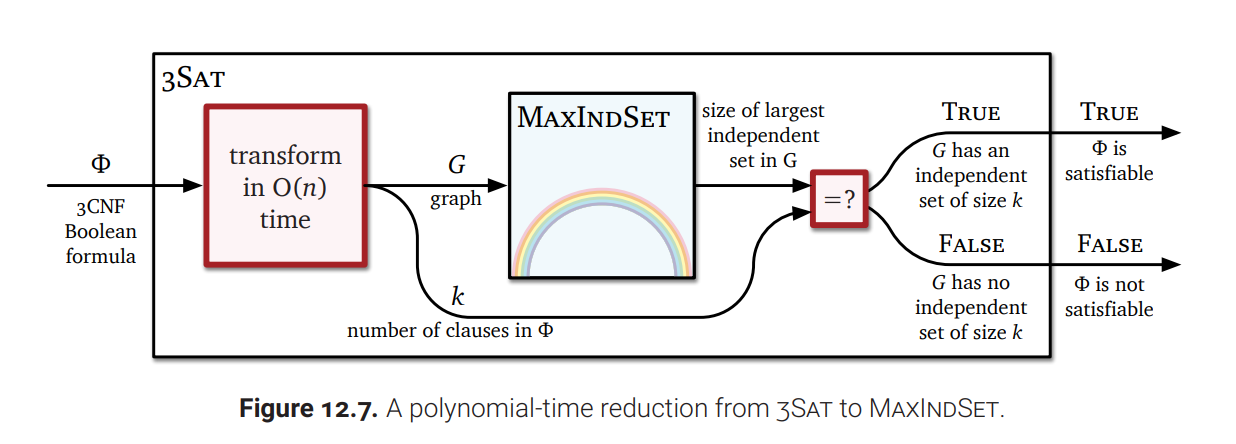
\includegraphics[width=.8\textwidth]{reduction.png}
    \end{center}
\end{frame}

\begin{frame}{Looking at Fine Grained Complexity}
    \begin{itemize}
        \item P vs NP is cool and all - but trodded ground \pause
        \item It's unlikely anyone will make meaningful progress other than showing problems are hard \pause
        \item But what about problems we know how to solve fast? \pause
        \item How fast can we solve these problems?
    \end{itemize}
\end{frame}

\begin{frame}{Looking at Fine Grained Complexity}
    \begin{itemize}
        \item FGC looks at complexity at a function level: Problems that are $O(n^2)$ and reducing between them. \pause
        \item The techniques of reductions still apply, but now if we're trying to show something is $O(n^2)$-hard, our reduction can't be slower than $O(n^2)$
        \item $O(n^2)$ is just an example, reductions between problems in P is the idea.
    \end{itemize}
\end{frame}

\begin{frame}{Leetcode Haunts Us}
    \begin{itemize}
        \item \textsc{TwoSum}: Given an array of $n$ numbers, find 2 numbers that sum to $t$ \pause 
        \item How do we solve it? \pause
        \item Iterate through, storing $t-i$ in a BST or Hashmap. $O(n \log n)$ or $O(n)$ expected.
    \end{itemize}
\end{frame}

\begin{frame}{Leetcode Haunts Us}
    \begin{itemize}
        \item \textsc{ThreeSum}: Given an array of $n$ numbers, find 3 numbers that sum to $0$ \pause 
        \item How do we solve it? \pause
        \item Iterate through, Calling \textsc{TwoSum} with the value at the given index as $t$, and the rest of the array \pause
        \item $O(n)$ calls to TwoSum, $O(n^2)$.
    \end{itemize}
\end{frame}

\begin{frame}{3SUM}
    \begin{itemize}
        \item Can we do better? \pause
        \item We... don't know! \pause 
        \item Using the same decision tree analysis as we did with sorting, Kane, Lovett and Moran showed \textsc{3SUM} has a $O(n\log^2(n))$ decision complexity \pause 
        \item No-one has been able to come up with a working sub-quadratic algorithm for the purely general case.
    \end{itemize}    
\end{frame}

\begin{frame}{3SUM}
\begin{itemize}

    \item This constant searching has led to the \textbf{\textit{3SUM Conjecture:}}
    \begin{itemize}
        \item There is no algorithm to solve \textsc{3SUM} in $O(n^{2-\epsilon})$ for $\epsilon > 0$ \pause
    \end{itemize}
    \item With this has led to a massive field of research, reductions, and discoveries
\end{itemize}    
\end{frame}

\begin{frame}{Geombase}
\begin{itemize}
    \item We turn to another problem, Geombase:
\end{itemize}
\begin{center}
    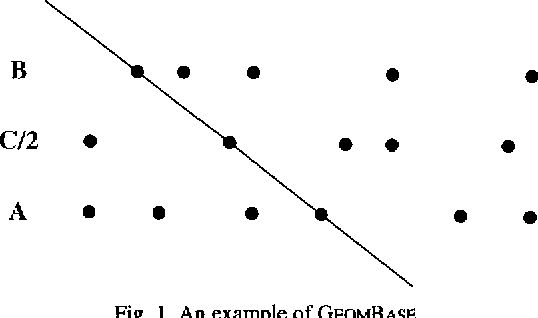
\includegraphics[width=.8\textwidth]{image.png}
\end{center}
\end{frame}

\begin{frame}{Geombase}
\begin{itemize}
    \item Given $n$ points on 3 parallel lines, is there 3 points that are co-linear across the 3 lines? \pause 
    \item We can show that this problem is \textsc{3SUM} hard!
\end{itemize}
\end{frame}

\begin{frame}{3SUM to Geombase}
\begin{itemize}
    \item Given $n$ points on 3 parallel lines, is there 3 points that are co-linear across the 3 lines? \pause 
    \item We can show that this problem is \textsc{3SUM} hard!
\end{itemize}
\end{frame}

\begin{frame}{3SUM to Geombase}
\begin{itemize}
    \item Equivalent 3SUM Problem: Given 3 arrays $A,B,C$ find one element in each such that $a+b+c=0$ \pause
    \item We take each element $a \in A$ and make a point $(2a,0)$, $b \in B$, $(2b,2)$, and $c \in C$, $(-c,1)$ \pause
    \item We see that a solution is finding three points $(x_i, 0), (x_j, 1), (x_k, 2)$ where $x_i + x_k = 2x_j$ \pause
    \item With the points we made, $2a + 2b = -2c \implies a + b + c = 0$ \pause
    \item This reduction took $O(n)$ time, thus Geombase is $3SUM$-Hard.
\end{itemize}
\end{frame}

\begin{frame}{Improvements to 3SUM}
    \begin{itemize}
        \item People still try to find better algorithms, because they are tractable! \pause
        \item In 2018 Timothy M Chan (Professor Here!) found a $O(n^2 (\log \log n)^{O(1)} / log^2(n))$ solution to 3SUM
        \item With certain assumptions, 3SUM can be solved relatively fast as well (such as a bounded universe).
    \end{itemize}
\end{frame}

\begin{frame}{Other Conjectures}
    \begin{itemize}
        \item All Pairs Shortest Path (APSP)
        \begin{itemize}
            \item Find the shortest path between all pairs of vertices \pause 
            \item We can reduce to matrix multiplication... $O(n^{\omega})$ for $\omega = 2.371522$ \pause
            \item Is there a \textit{combinatorial} algorithm $O(n^{3-\epsilon})$?
        \end{itemize}
        \item Orthogonal Vectors (OV)
        \begin{itemize}
            \item Given two sets of bitvectors of size $d$, find a pair for which $a \cdot b = \mathbf{0}$
            \item $O(dn^2)$, $O(4^d + n)$ (when $d$ is small). \pause 
            \item Conjecture: No $O(n^{2- \epsilon})$ when $d >> \log(n)$
        \end{itemize}
    \end{itemize}
\end{frame}

\begin{frame}{Connections to NP}
    \begin{itemize}
        \item Orthogonal Vectors (OV) has a reduction from $k$-SAT! \pause 
        \begin{itemize}
            \item Suppose a $O(d^{O(1)}n^{2 - \epsilon})$ algorithm existed for OV... \pause 
            \item Through some care, we can take a $k$-CNF Boolean Formula and turn it into two sets of size $2^{(n/2)}$. \pause
            \item Then we can solve $k$-SAT in $O^*(2^{(1-\epsilon/2)n})$ time! \pause 
            \item $O^*( \cdot )$ hides polynomial factors.
        \end{itemize}
    \end{itemize}
\end{frame}

\begin{frame}{}
      \begin{center}
    {\color{sigma@mainblue} \LARGE Questions?}
  \end{center}
\end{frame}

% \begin{frame}{Updates!}
%   % Let's put some real content in this frame:
%   Weekly updates:
%   \begin{itemize}
%     \item SIGma is an excellent SIG.
%     \item I'm out of ideas for updates.
%   \end{itemize}
% \end{frame}

% % Start a section: *sections* (subsections, etc.) are what show up in the TOC.
% \section{Basics}
% % Section pages can be printed thus:
% \frame{\sectionpage}
% % There's a way to automate this, see:
% % https://tex.stackexchange.com/questions/178800/creating-sections-each-with-title-pages-in-beamers-slides/178803

% \begin{frame}{Some Text}
%     \begin{itemize}
%         \item You may want some stuff to appear in a sequence \pause
%         \item Use \textbackslash pause for this \pause
%         \item \textcolor{sigma@mainblue}{colors} \textcolor{sigma@highlightpink}{are} \textcolor{sigma@alertred}{cool}
%     \end{itemize}
% \end{frame}

% \begin{frame}
%   \frametitle{Some Math Mode Testing}
%   % Some fun with LaTeX Math
%   $$\frac{x^2+3}{y^2+7}$$

%   \[
%     \mathcal L_{\mathcal T}(\vec{\lambda})
%     = \sum_{(\mathbf{x},\mathbf{s})\in \mathcal T}
%        \log P(\mathbf{s}\mid\mathbf{x}) - \sum_{i=1}^m
%        \frac{\lambda_i^2}{2\sigma^2}
%   \]

%   $$\int_0^8 f(x) dx$$
% \end{frame}

% % Use \pause to make stuff readable
% % Large walls of text scare the audience, we don't want that
% % Introducing stuff sequentially allows for questions
% \begin{frame}
%   % Alternate syntax for frame titles
%   \frametitle{There Is No Largest Prime Number}
%   % Frames can have subtitles:
%   \framesubtitle{The proof uses \textit{reductio ad absurdum}.}
%   % Some frame content:
%   \begin{thrm}
%     There is no largest prime number.
%   \end{thrm}
%   \begin{pf}
%     \begin{enumerate}
%         \item Suppose $p$ were the largest prime number \pause
%         \item Let $q$ be the product of the first $p$ primes \pause
%         \item Then $q+1$ is not divisible by any of them \pause
%         \item But $q + 1$ is greater than $1$, thus divisible by some prime number not in the first $p$ numbers. \pause
%         \item Thus, there exists a prime larger than $p$.
%     \end{enumerate}
%   \end{pf}
% \end{frame}

% % However, this doesn't work in math mode. It is quite annoying to figure out
% % So just copy this as reference
% % This works for \onslide<> and \item<>
% % Really good read on this: 
% %   https://www.texdev.net/2014/01/17/the-beamer-slide-overlay-concept/
% \begin{frame}{Sequential Math Frames}
%     Here is a sentence \pause
    
%     I shall now carry out some calculations \pause
%     \begin{align*}
%         \onslide<+->{\zeta(s) &= \sum_{n = 1}^\infty \frac{1}{n^s} \\}
%         \onslide<+->{&= \prod_{p \in \text{primes}} \frac{1}{1 - p^{-s}} \\}
%         \onslide<.->{&= \frac{1}{1 - 2^-s} \cdot \frac{1}{1 - 3^-s} \cdots \\}
%         \onslide<+->{&= \frac{1}{\Gamma(s)} \int_0^\infty \frac{x^{s - 1}}{e^x - 1} ~\textrm{d}x\\}
%     \end{align*}
% \end{frame}

% \section{Some Template Slides}
% \frame{\sectionpage}

% % Similar for subsections:
% \subsection{A subsection, Wow}
% % And their pages:
% \frame{\subsectionpage}

% \begin{frame}{Image}
%   % This is how you'd include an image, centered.
%   \begin{center}
%     
\includegraphics[width=0.25\textwidth]{sigma.png}
%   \end{center}
% \end{frame}

% \begin{frame}{Side by Side}
%     
\includegraphics[width=0.25\textwidth]{sigma.png}\hspace{0.4\textwidth}
%     
\includegraphics[width=0.25\textwidth]{sigma.png}
% \end{frame}

% \begin{frame}{Demonstration of algo and nalgo env}
%     \begin{algo}
%     \underline{\textsc{GetRandomNumber}():}\+
%     \\      return $4$   \Comment{chosen by fair dice roll.}
%     \\      \hspace{42.75pt}\Comment{guaranteed to be random.}
%     \end{algo}
    
%     % nalgo has line numbers
%     % only lines with \label{} are numbered
%     \begin{nalgo}[1.3]
%         \underline{\textsc{GetRandomNumber}():}\+
%     \\\label{}  return $4$   \Comment{chosen by fair dice roll.}
%     \\\label{}  \hspace{42.75pt}\Comment{guaranteed to be random.}
%     \end{nalgo}
    
%     Random number generation from~\cite{site:xkcd}. 
%     \quest{
%     \textbackslash cref for line numbers does not work. 
%     If you want to refer to specific line numbers, do it manually
%     }
    
% \end{frame}

% \begin{frame}{}
% \begin{minipage}[c]{0.6\textwidth}
% \begin{nalgo}
% \textul{\textbf{\textsc{AlgorithmP}}$(S[a_0, \dots, a_n])$}:
% \\\label{}  $C[1..n] \gets 0, O[1..n] \gets 1$
% \\\label{}  \textbf{while} \textsc{True}:\+
% \\\label{}      \textsc{print}$(S)$
% \\\label{}      {\color{lightgray}$j \gets n, s \gets 0$}
% \\\label{}      {\color{lightgray}\textbf{A:}~~$q \gets C[j] + O[j]$\+}
% \\\label{}          {\color{lightgray}\textbf{if} $q < 0$: goto \textbf{D}}
% \\\label{}          {\color{lightgray}\textbf{if} $q = j$: goto \textbf{B}}
% \\\label{}          {\color{lightgray}\textsc{swap}$(S, j-C[j]+s, j-q+s)$}
% \\\label{}          {\color{lightgray}$C[j] \gets q$} 
% \\\label{}          {\color{lightgray}continue\-}
% \\\label{}      {\color{lightgray}\textbf{B:}~~\textbf{if} $j=1$:\+\+}
% \\\label{}              {\color{lightgray}break\-}
% \\\label{}          {\color{lightgray}$s \gets s+1$\-}
% \\\label{}    {\color{lightgray}\textbf{D:}~~$O[j] \gets -O[j], j \gets j-1$\+}
% \\\label{}      {\color{lightgray}goto \textbf{A}}
% \end{nalgo}
% \end{minipage}
% \begin{minipage}[c]{0.35\textwidth}
% \begin{itemize}
%     \item Here is an example of annotating an algorithms \pause
%     \item We have grayed out text to highlight what we want to discuss 
% \end{itemize}
% \end{minipage}
% \end{frame}

% % Of course, not everything is in pseudocode
% % You MUST have this [containsverbatim] option
% % https://www.overleaf.com/learn/latex/Code_Highlighting_with_minted
% \begin{frame}[containsverbatim]{Source Code}
%     \begin{minted}
%     [
%     framesep=2mm,
%     baselinestretch=1.2,
%     bgcolor=black,
%     fontsize=\footnotesize,
%     ]
%     {python}
%     def algorithm_g(n):
%         a = [0 for _ in range(n + 1)]
%         while True:
%             curr = a[1 : n + 1][::-1]
%             yield "".join([str(i) for i in curr])
    
%             a[0] = 1 - a[0]
%             j = 1
%             while a[j - 1] != 1:
%                 j += 1
%             if j == n + 1:
%                 return
%             a[j] = 1 - a[j]
%     \end{minted}
% \end{frame}


% \begin{frame}{Theorems and Lemmas}
%     \begin{lem}
%         The map $\C \times \pqty{\C \setminus \set{0}} \to \C$, $(z, w) \mapsto z / w$ is $C^{\infty}$.
%     \end{lem}
%     \begin{pf}
%         To see this, we identify $\C$ with $\R^{2}$ where $a + bi = (a, b)$.
%         Thus our map is now
%         \begin{align*}
%             \pqty{\R^{2}} \times \pqty{\R^{2} \setminus \set{(0, 0)}} &\to \R^{2} \\
%                             ((a, b), (c, d)) &\mapsto \pqty{\frac{ac + bd}{c^{2} + d^{2}}, \frac{bc - ad}{c^{2} + d^{2}}}
%         \end{align*}
%         which is well defined since at least one of $c$ or $d$ is nonzero.
%         It is simple to verify that this map is equivalent to the original one.
%         Since this new map is $C^{\infty}$ in each component, we have that it is $C^{\infty}$ overall.
%     \end{pf}
% \end{frame}

% \section{Conclusion}
% \frame{\sectionpage}

% % Asking questions is fun but we should answer some first
% \begin{frame}{}
%       \begin{center}
%     {\color{sigma@mainblue} \LARGE Questions?}
%   \end{center}
% \end{frame}

% \begin{frame}{Questions!}
%     \begin{itemize}
%         \item How many zeros of $\zeta(s) = \sum\limits_{i = 1}^\infty \frac{1}{n^s} = \prod\limits_{p \text{ prime}} \frac{1}{1 - p^{-s}}$ have real part equal to $\frac{1}{2}$?
%         \item Find a closed form to the following recurrence:
%         $$
%             f(n) = \begin{cases} 
%                 f\pqty{\frac{n}{2}} & n \text{ even} \\
%                 f{3n + 1} & \text{otherwise}                
%             \end{cases}
%         $$
%     \end{itemize}
% \end{frame}

% % Quotes are fun, find some to use!
% \font\eightss=cmssq8
% \font\eightssi=cmssqi8
% \newcommand\quoteAuthorDate[3]{\begingroup
%   \baselineskip 10pt
%   \parfillskip 0pt
%   \interlinepenalty 10000 % not needed in example
%   \leftskip 0pt plus 40pc minus \parindent
%   \let\rm=\eightss
%   \let\sl=\eightssi
%   \everypar{\sl}#1\par
%   \nobreak\smallskip
%   \noindent\rm--- #2\unskip\enspace(#3)\par
%   \endgroup}
% % If someone can figure out how to horizontally center this and make the text bigger that'd be cool
% \begin{frame}
%     \begin{center}
%         \item \quoteAuthorDate{So long and thanks for all the fish!}{DOUGLAS ADAMS}{\textcolor{sigma@mainblue}{1979}}
%     \end{center}
% \end{frame}

% % Remove this slide if you came up with all the material yourself
% \begin{frame}[allowframebreaks]{Bibliography}
%     \tiny
%     \bibliography{refs}
%     \bibliographystyle{alpha}
% \end{frame}

\end{document}